% !TeX spellcheck = en_US
% !TeX encoding = utf8
% !TeX program = xelatex
% !BIB program = bibtex

% \documentclass[mathserif,compress,12pt]{ctexbeamer}
\documentclass[12pt,notes,mathserif]{beamer}
% \documentclass[draft]{beamer}	
\usetheme{Singapore}
% \usetheme{Hannover}
%\usepackage{pgfpages}
%\setbeameroption{show notes on second screen}

\usepackage[british]{babel}
\usepackage{graphicx,hyperref,url}
% \usepackage{ru}
\usepackage{mmstyles,bm,ulem}
\usepackage{multirow}
\usepackage{listings}
\usefonttheme[onlymath]{serif}
\usepackage{fontspec}
\usepackage{xeCJK}
% \pgfdeclareimage[width=\paperwidth,height=\paperheight]{bg}{background}
% \setbeamertemplate{background}{\pgfuseimage{bg}}
%% columns
\newcommand{\begincols}[1]{\begin{columns}{#1}}
\newcommand{\stopcols}{\end{columns}}
% \usepackage[backend=biber]{biblatex}
% \bibliography{./ref.bib}
%\addbibresource{ref.bib}
\usepackage{indentfirst}
\usepackage{longtable}
\usepackage{float}
%\usepackage{picins}
\usepackage{rotating}
\usepackage{subfigure}
\usepackage{tabu}
\usepackage{amsmath}
\usepackage{amssymb}
\usepackage{setspace}
\usepackage{amsfonts}
\usepackage{appendix}
\usepackage{listings}
\usepackage{colortbl}
\usepackage{geometry}
\usepackage{xcolor}

% \setCJKfamilyfont{cjkhwxk}{SimSun}
% \newcommand*{\cjkhwxk}{\CJKfamily{cjkhwxk}}
%\newfontfamily{\consolas}{Consolas}
%\newfontfamily{\monaco}{Monaco}
%\setmonofont[Mapping={}]{Consolas}	%英文引号之类的正常显示,相当于设置英文字体
%\setsansfont{Consolas} %设置英文字体 Monaco, Consolas,  Fantasque Sans Mono
% \setmainfont{Times New Roman}
% \newfontfamily{\consolas}{Times New Roman}
% \newfontfamily{\monaco}{Arial}
% \setCJKmainfont{Times New Roman}
%\setmainfont{MONACO.TTF}
%\setsansfont{MONACO.TTF}
\newcommand{\verylarge}{\fontsize{60pt}{\baselineskip}\selectfont}  
\newcommand{\chuhao}{\fontsize{44.9pt}{\baselineskip}\selectfont}  
\newcommand{\xiaochu}{\fontsize{38.5pt}{\baselineskip}\selectfont}  
\newcommand{\yihao}{\fontsize{27.8pt}{\baselineskip}\selectfont}  
\newcommand{\xiaoyi}{\fontsize{25.7pt}{\baselineskip}\selectfont}  
\newcommand{\erhao}{\fontsize{23.5pt}{\baselineskip}\selectfont}  
\newcommand{\xiaoerhao}{\fontsize{19.3pt}{\baselineskip}\selectfont} 
\newcommand{\sihao}{\fontsize{14pt}{\baselineskip}\selectfont}      % 字号设置  
\newcommand{\xiaosihao}{\fontsize{12pt}{\baselineskip}\selectfont}  % 字号设置  
\newcommand{\wuhao}{\fontsize{10.5pt}{\baselineskip}\selectfont}    % 字号设置  
\newcommand{\xiaowuhao}{\fontsize{9pt}{\baselineskip}\selectfont}   % 字号设置  
\newcommand{\liuhao}{\fontsize{7.875pt}{\baselineskip}\selectfont}  % 字号设置  
\newcommand{\qihao}{\fontsize{5.25pt}{\baselineskip}\selectfont}    % 字号设置 


\newcommand{\red}[1]{ {\color{red}{#1}} }

\graphicspath{{./fig/}}

% \setbeamertemplate{footnote}{%
%   \hangpara{2em}{1}%
%   \makebox[2em][l]{\insertfootnotemark}\footnotesize\insertfootnotetext\par%
% }

\definecolor{cred}{rgb}{0.6,0,0}
\definecolor{cgreen}{rgb}{0.25,0.5,0.35}
\definecolor{cpurple}{rgb}{0.5,0,0.35}
\definecolor{cdocblue}{rgb}{0.25,0.35,0.75}
\definecolor{cdark}{rgb}{0.95,1.0,1.0}
\lstset{
	language=R,
	numbers=left,
	numberstyle=\tiny\color{black},
	keywordstyle=\color{cpurple}\consolas,
	commentstyle=\color{cgreen}\consolas,
	stringstyle=\color{cred}\consolas,
	frame=single,
	escapeinside=``,
	xleftmargin=1em,
	xrightmargin=1em, 
	backgroundcolor=\color{cdark},
	aboveskip=1em,
	breaklines=true,
	tabsize=3
} 

\providecommand{\tightlist}{%
  \setlength{\itemsep}{0pt}\setlength{\parskip}{0pt}}

  
% The title of the presentation:
%  - first a short version which is visible at the bottom of each slide;
%  - second the full title shown on the title slide;
% \title[]{\LARGE CSE 5526: Introduction to Neural Networks}
\title{Support Vector Machines (SVM)}

% Optional: a subtitle to be dispalyed on the title slide
% \subtitle{\Large Support Vector Machines
% (SVM)}

% The author(s) of the presentation:
%  - again first a short version to be displayed at the bottom;
%  - next the full list of authors, which may include contact information;
\author[YingmingLi]{Yingming Li \\ yingming@zju.edu.cn}
% The institute:
%  - to start the name of the university as displayed on the top of each slide
%    this can be adjusted such that you can also create a Dutch version
%  - next the institute information as displayed on the title slide

\institute[DSERC, ZJU]{Data Science \& Engineering Research Center, ZJU}
% Add a date and possibly the name of the event to the slides
%  - again first a short version to be shown at the bottom of each slide
%  - second the full date and event name for the title slide
\date[\today]{\today}
\begin{document}

\AtBeginSection[]
{
	\begin{frame}
		\frametitle{Outline}
		\tableofcontents[currentsection]
	\end{frame}
}

% \AtBeginSubsection[2-]
% {
%    \begin{frame}
%        \frametitle{Outline}
%        \tableofcontents[currentsection]
%    \end{frame}
% }
\begin{frame}[c]
	\titlepage
	\begin{center}
		Adapted from slides provided by Prof. Michael Mandel.
	\end{center}
\end{frame}

% 2
\begin{frame}[c]
	\frametitle{Perceptrons find any separating hyperplane}
	\begin{center}
		Depends on initialization and ordering of training points\\
		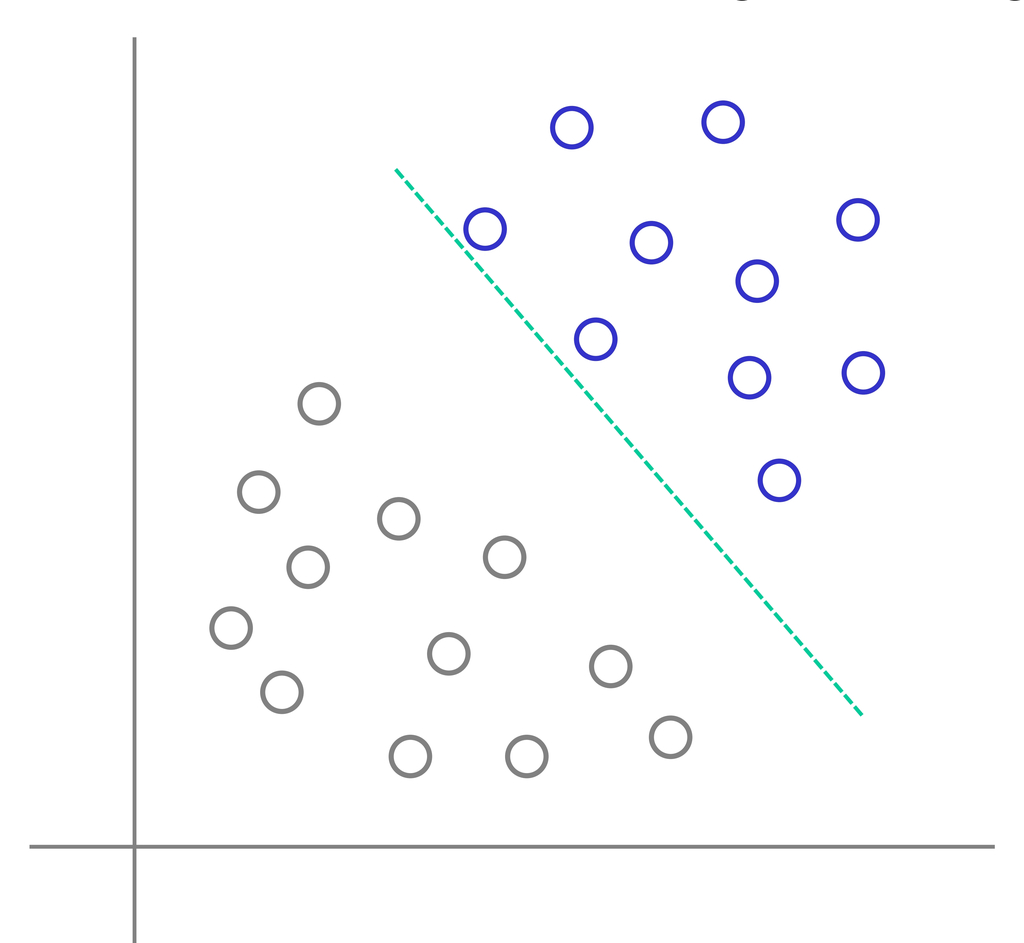
\includegraphics[width=0.7\linewidth]{fig8/lec82.jpg}
	\end{center}
\end{frame}
% 3
\begin{frame}[c]
	\frametitle{Perceptrons find any separating hyperplane}
	\begin{center}
		Depends on initialization and ordering of training points\\
		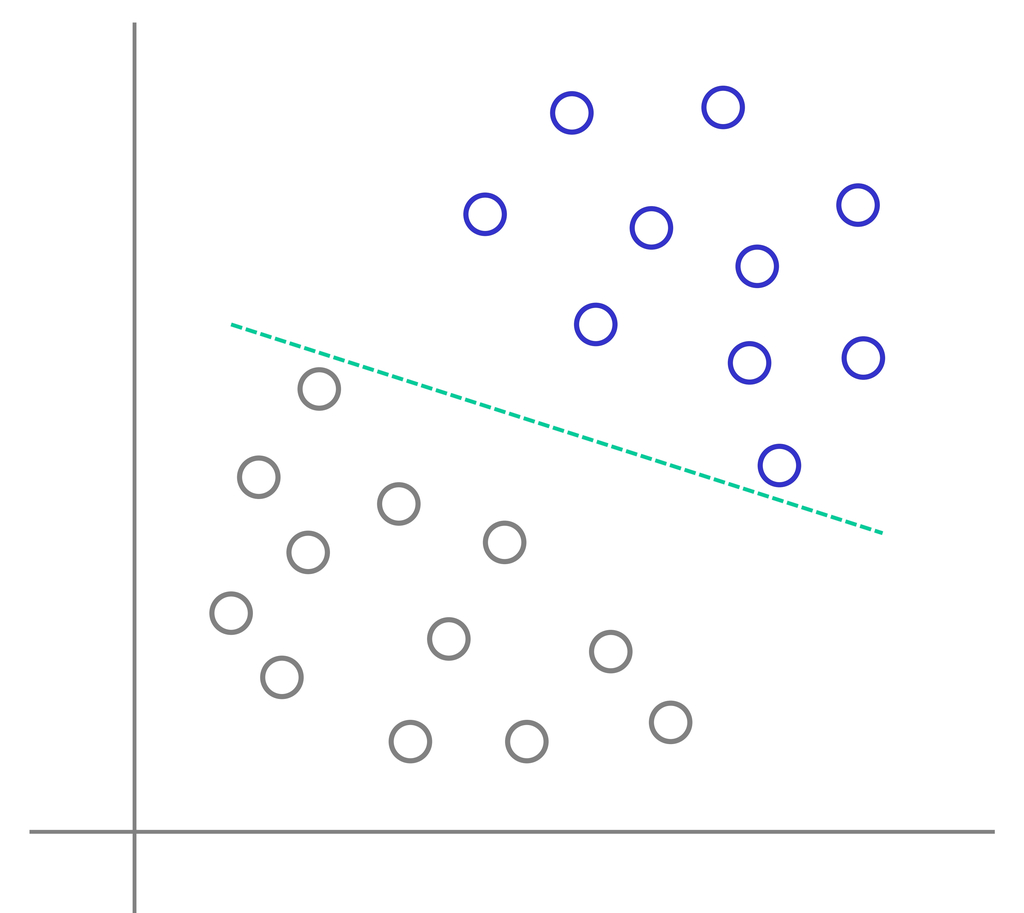
\includegraphics[width=0.7\linewidth]{fig8/lec83.jpg}
	\end{center}
\end{frame}

% 4
\begin{frame}[c]
	\frametitle{Perceptrons find any separating hyperplane}
	\begin{center}
		Depends on initialization and ordering of training points\\
		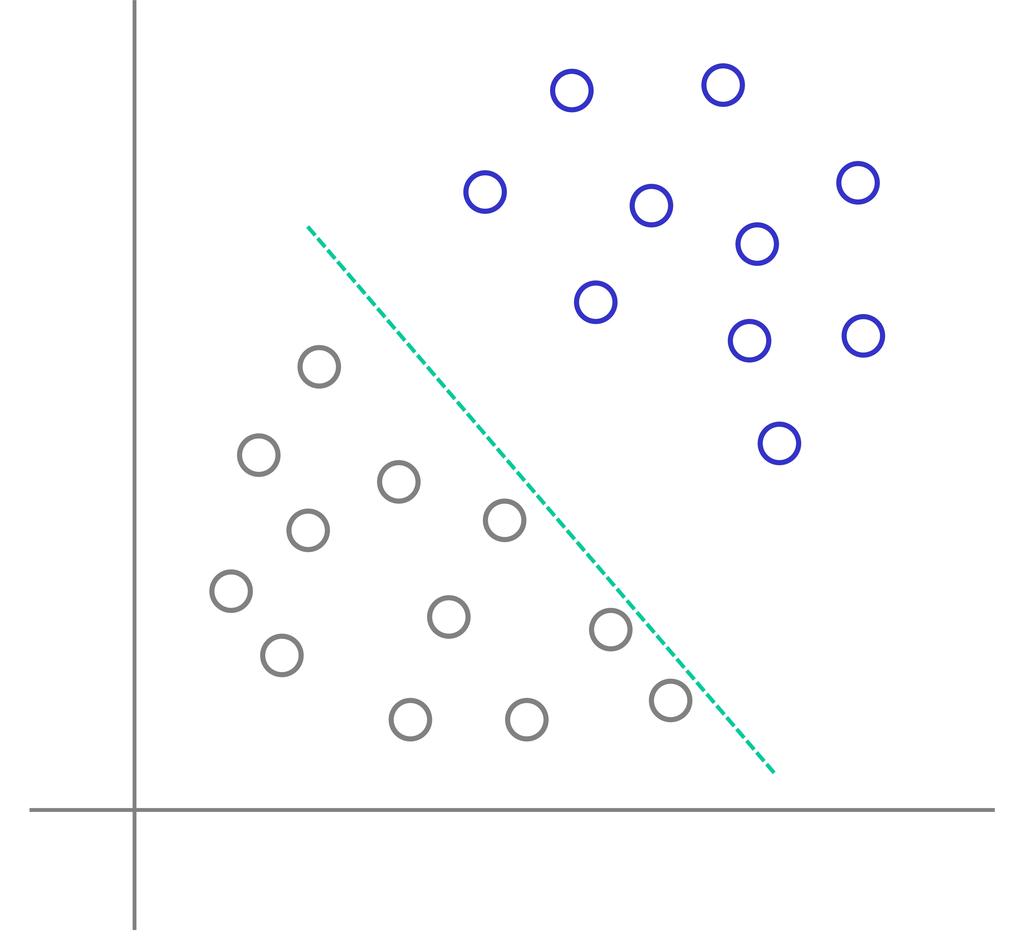
\includegraphics[width=0.7\linewidth]{fig8/lec84.jpg}
	\end{center}
\end{frame}

% 5
\begin{frame}[c]
	\frametitle{Perceptrons find any separating hyperplane}
	\begin{center}
		Depends on initialization and ordering of training points\\
		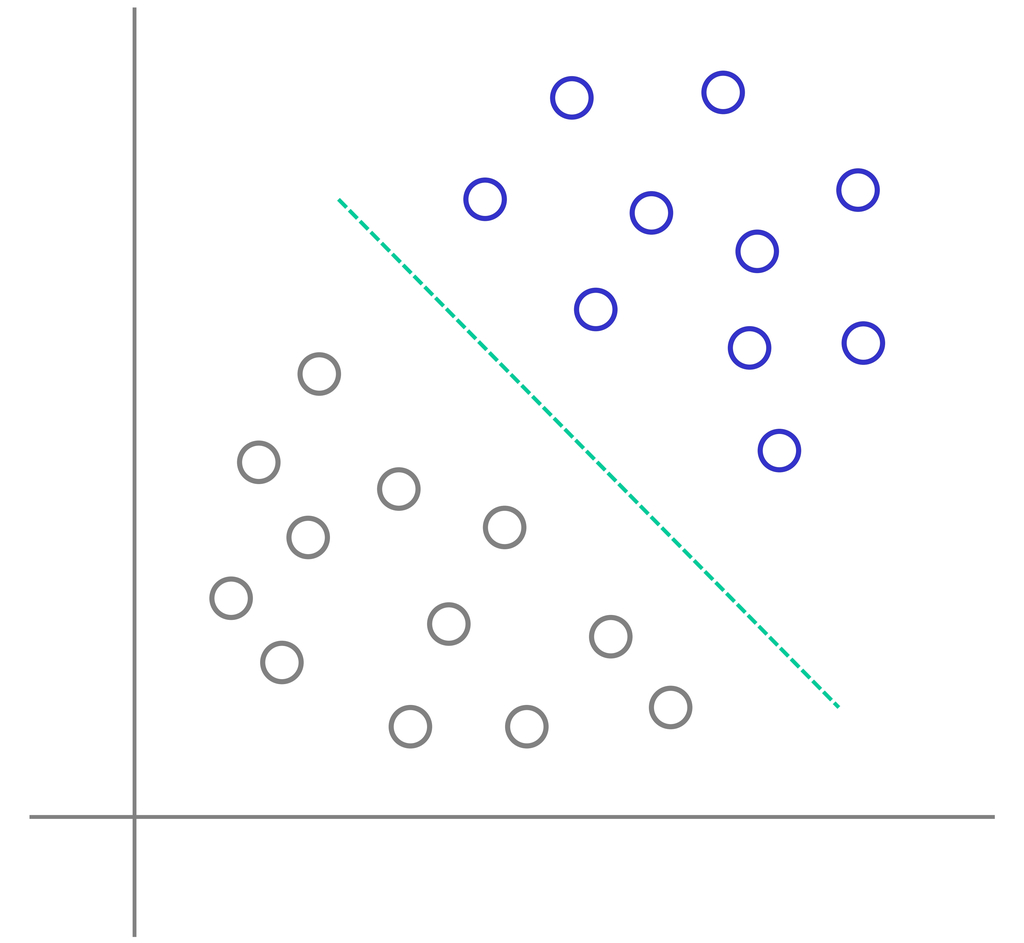
\includegraphics[width=0.7\linewidth]{fig8/lec85.jpg}
	\end{center}
\end{frame}



% 6
\begin{frame}[c]
	\frametitle{But the maximum margin hyperplane generalizes the best to new data}
	\begin{center}
		According to computational/statistical learning theory\\
		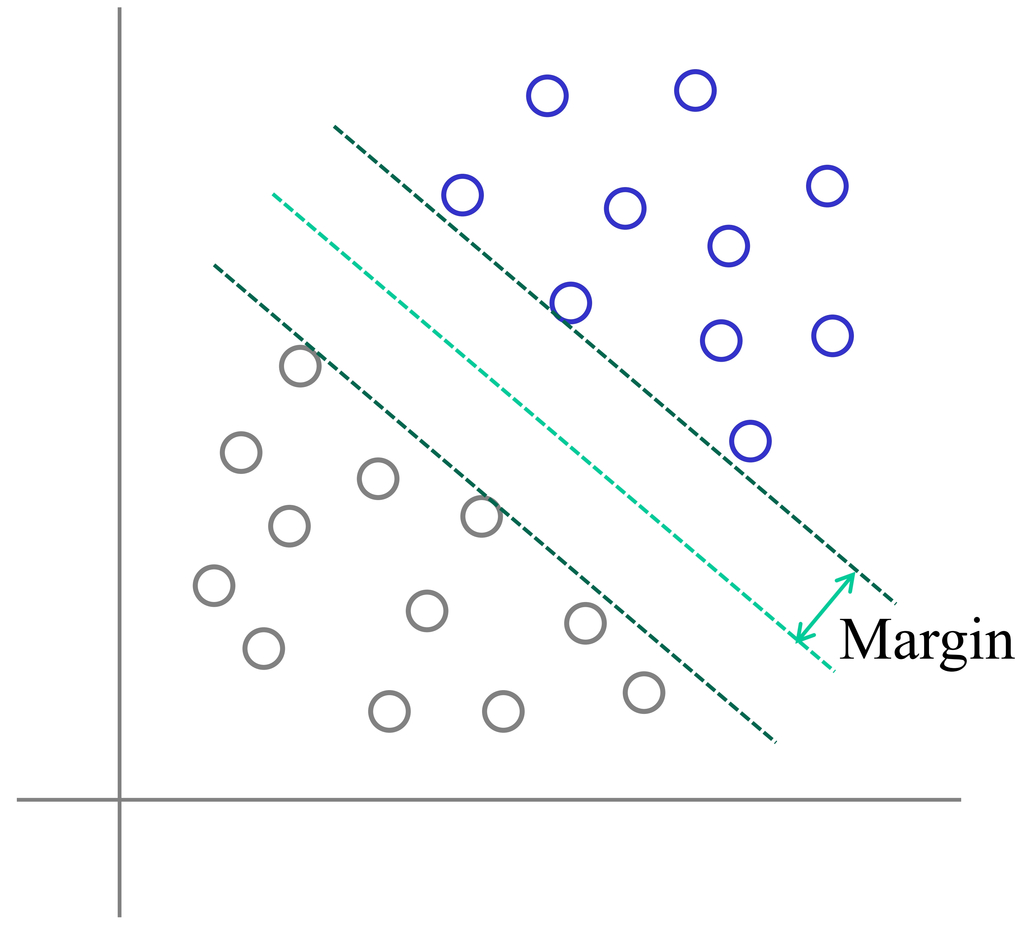
\includegraphics[width=0.6\linewidth]{fig8/lec86.jpg}
	\end{center}
\end{frame}


% 7
\begin{frame}[c]
	\frametitle{But the maximum margin hyperplane generalizes the best to new data}
	\begin{itemize}
		\item According to computational learning theory
		\item Also known as statistical learning theory
		\item We won't get into the details of that
		\item Recall from the perceptron convergence proof
		      \begin{itemize}
			      \item We assumed the existance of a best hyperplane $\mathbf{w}_0$
			      \item Which provided the maximum margin ${\alpha}$
			      \item Such that $d_p\mathbf{w}_0^T\mathbf{x}_p\leqslant{}\alpha$ for all training points $p$
		      \end{itemize}
		\item The SVM actually finds this hyperplane
	\end{itemize}

\end{frame}



% 8
\begin{frame}[c]
	\frametitle{The maximum margin only depends on certain points, the support vectors}
	\begin{center}
		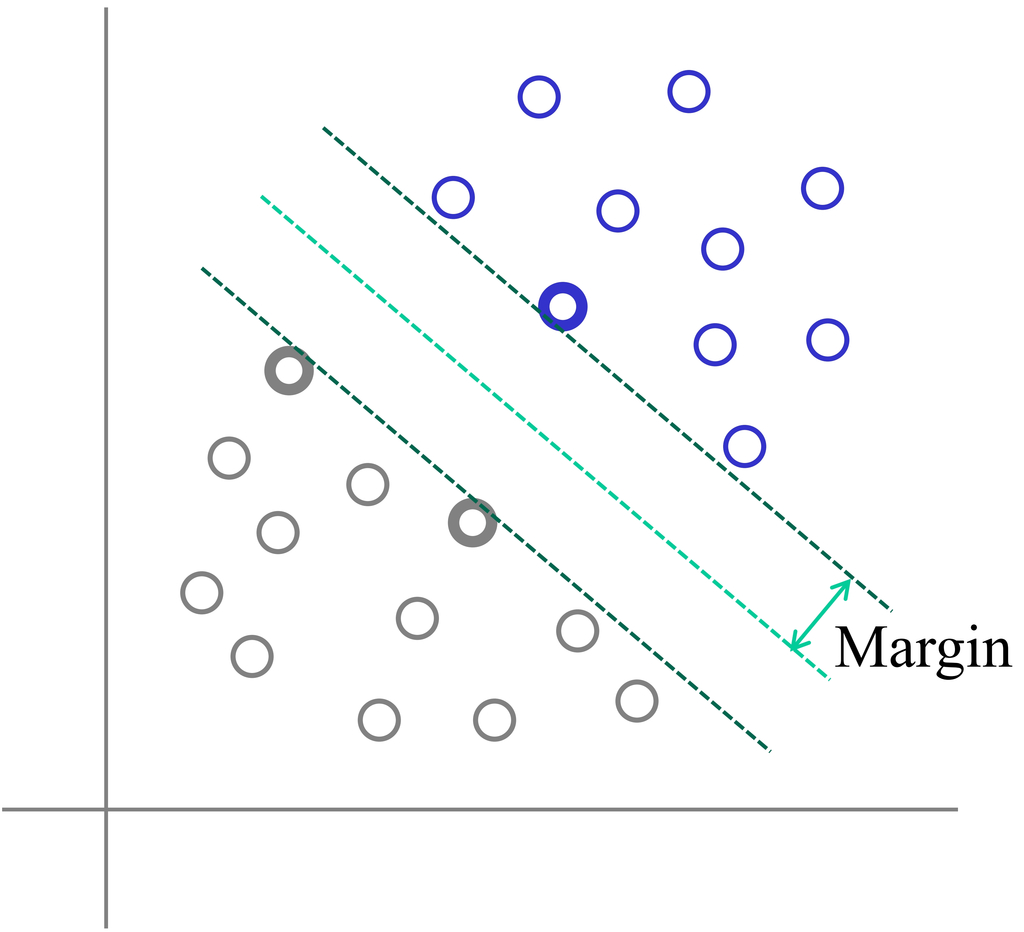
\includegraphics[width=0.7\linewidth]{fig8/lec88.jpg}
	\end{center}
\end{frame}

% 9
\begin{frame}[c]
	\frametitle{The maximum margin only depends on certain points, the support vectors}
	\begin{center}
		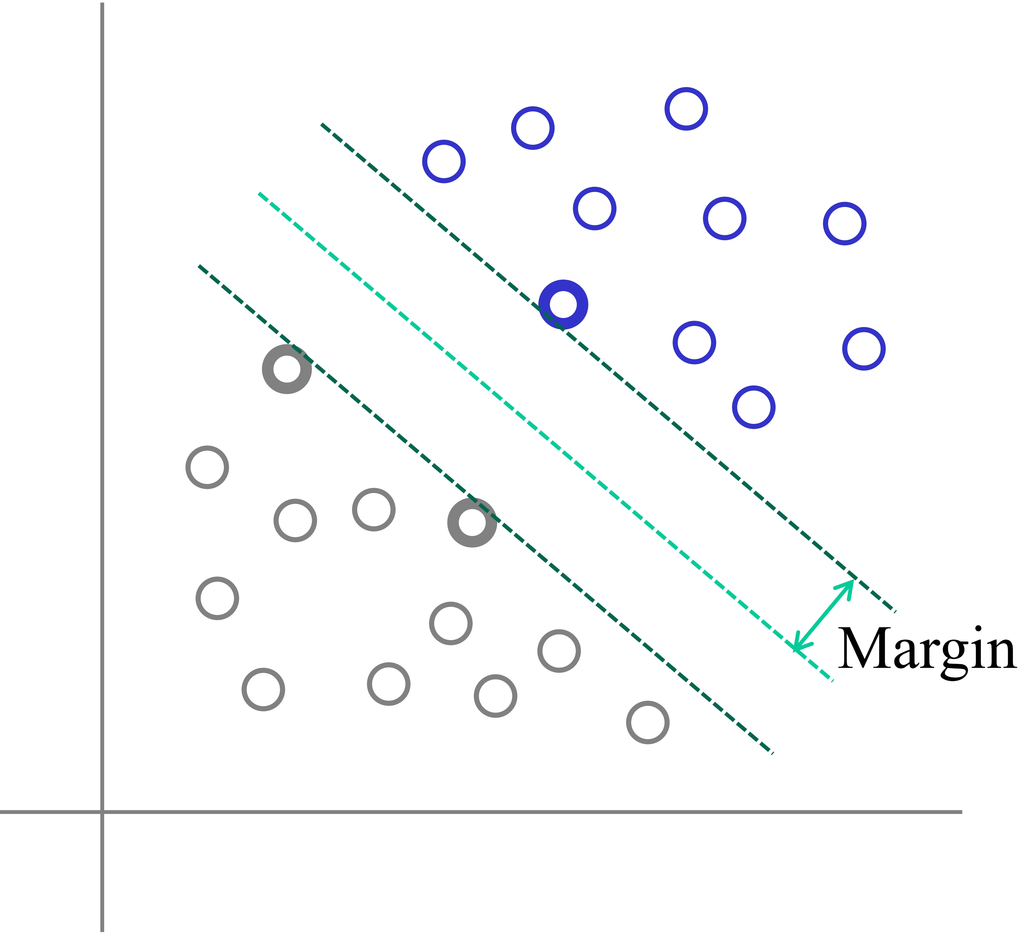
\includegraphics[width=0.7\linewidth]{fig8/lec89.jpg}
	\end{center}
\end{frame}


% 10
\begin{frame}[c]
	\frametitle{The maximum margin only depends on certain points, the support vectors}
	\begin{center}
		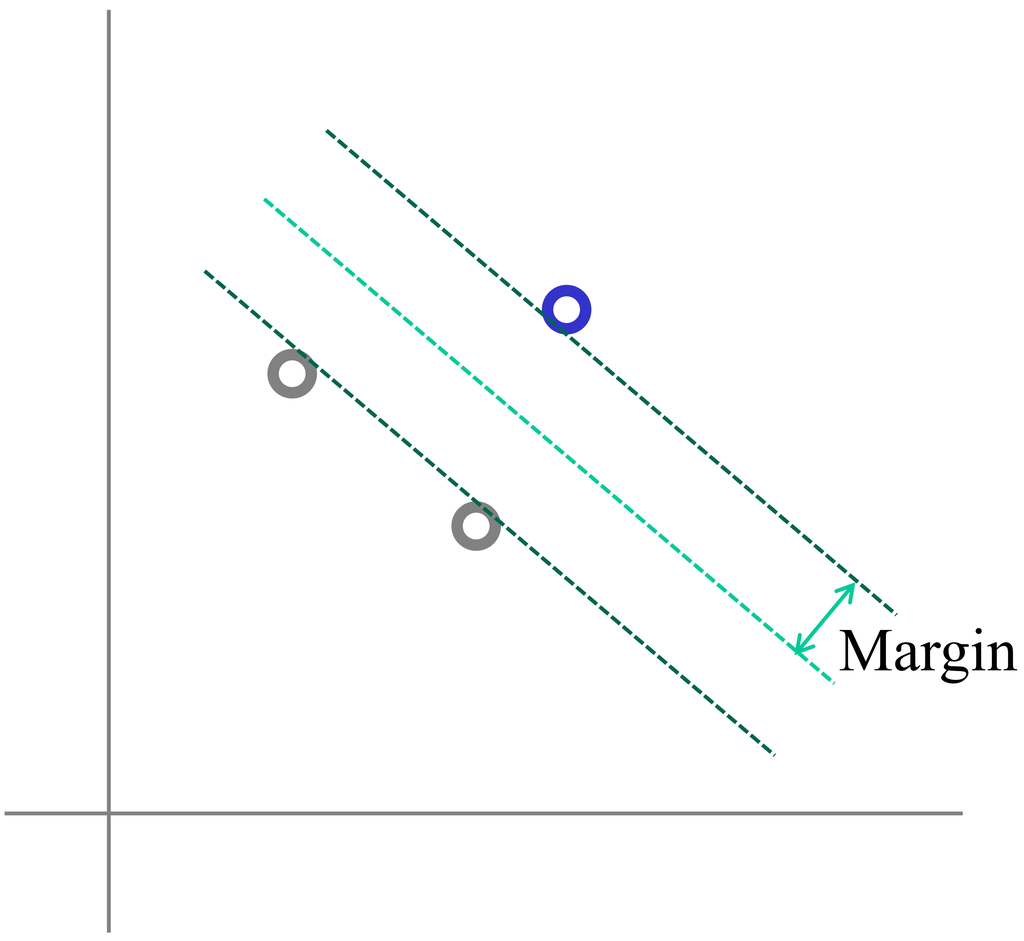
\includegraphics[width=0.7\linewidth]{fig8/lec810.jpg}
	\end{center}
\end{frame}


% 11
\begin{frame}[c]
	\frametitle{Maximum margin problem}
	\begin{itemize}
		\item  Given a set of data from two classes $\{\mathbf{x}_p,d_p\}$
		      \begin{itemize}
			      \item $\vx_p\in \mathbb{R}^D$ and $d_p\in\{-1,1\}$
			      \item Assume the classes are linearly separable for now
		      \end{itemize}
		\item Find the hyperplane that separates them
		      \begin{itemize}
			      \item with maximum margin
		      \end{itemize}
		\item Equation of general linear discriminant function
		      \[y(\mathbf{x})=\mathbf{w}^T\mathbf{x}+b\]

		\item Find $\mathbf{w}$ and $b$ that give maximum margin
		\item How can we quantify margin?
	\end{itemize}

\end{frame}



% 12
\begin{frame}[c]
	\frametitle{$\mathbf{w}$ is perpendicular to the hyperplane, $b$ defines its distance from the origin}
	\begin{center}
		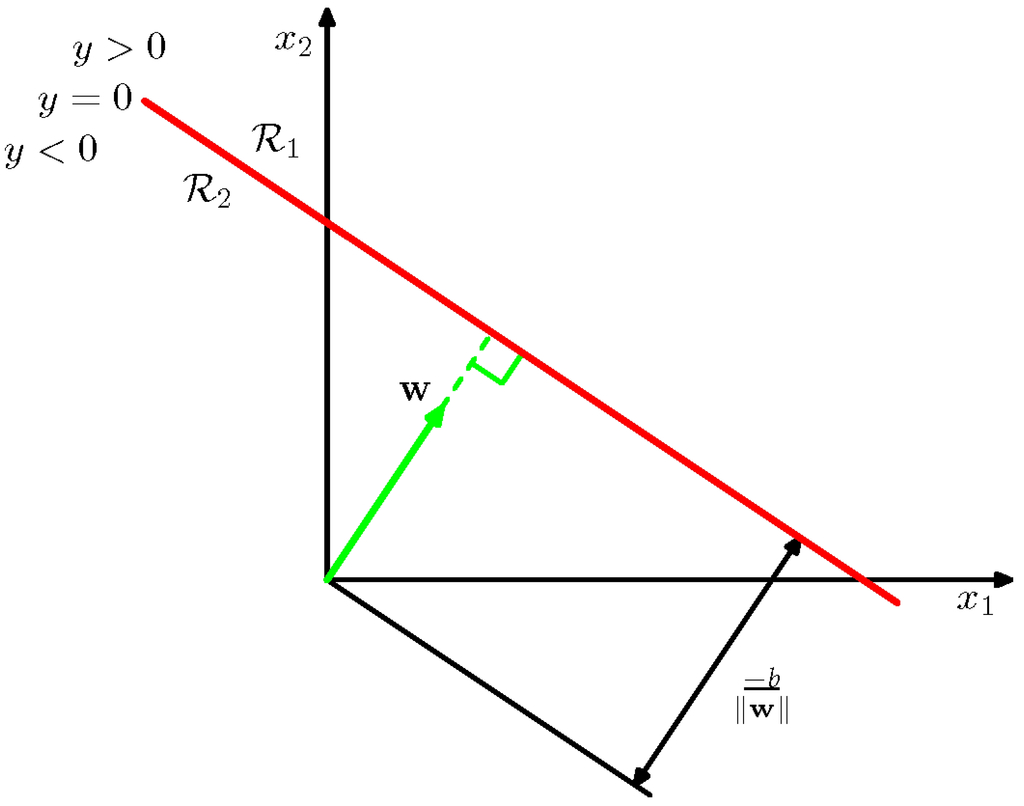
\includegraphics[width=0.7\linewidth]{fig8/lec812.jpg}
	\end{center}
\end{frame}


% 13
\begin{frame}[c]
	\frametitle{$\mathbf{w}$ is perpendicular to the hyperplane}
	\begin{itemize}
		\item Consider two points on the hyperplane $\mathbf{x}_A$ and $\mathbf{x}_B$
		\item Then $y(\mathbf{x}_A)=y(\mathbf{x}_B)=0$ by definition
		\item So $0 =y(\mathbf{x}_A)− y(\mathbf{x}_B) = \mathbf{w}^T(\mathbf{x}_A-\mathbf{x}_B)$𝒙𝒙 𝐵𝐵
		\item $\mathbf{x}_A-\mathbf{x}_B$ is  a vector pointing along the hyperplane
		\item So $\mathbf{w}$ is perpendicular to the hyperplane
	\end{itemize}

\end{frame}





% 14
\begin{frame}[c]
	\frametitle{$b$ defines the hyerplane's distance from the origin}
	\begin{itemize}
		\item Consider a general point $\mathbf{x}$
		\item Its distance to the origin is $D=\dfrac{\mathbf{w}^Tx}{||\mathbf{w}||}$
		\item If $\mathbf{x}$ is on the hyperplane, then $y(\mathbf{x})=0$
		      \begin{itemize}
			      \item So $\mathbf{w}^T x=-b$
		      \end{itemize}
		\item So the distance from the hyperplane to the origin is
		      \[
			      D=-\dfrac{b}{||\mathbf{w}||}
		      \]
	\end{itemize}

\end{frame}



% 15
\begin{frame}[c]
	\frametitle{$\mathbf{w}$ is perpendicular to the hyperplane, $b$ defines its distance from the origin}
	\begin{center}
		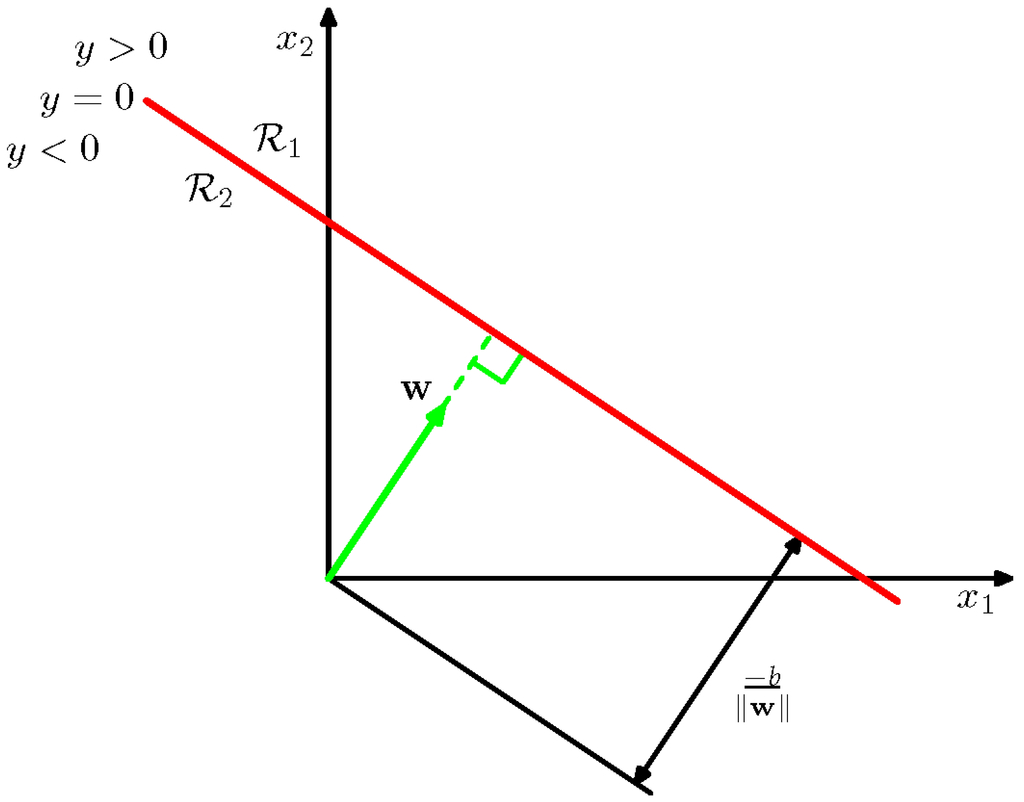
\includegraphics[width=0.7\linewidth]{fig8/lec815.jpg}
	\end{center}
\end{frame}


% 16
\begin{frame}[c]
	\frametitle{The distance from point $\mathbf{x}$𝒙to the hyperplane is 𝑦$y(\mathbf{x})/||\mathbf{w}||$}
	\begin{center}
		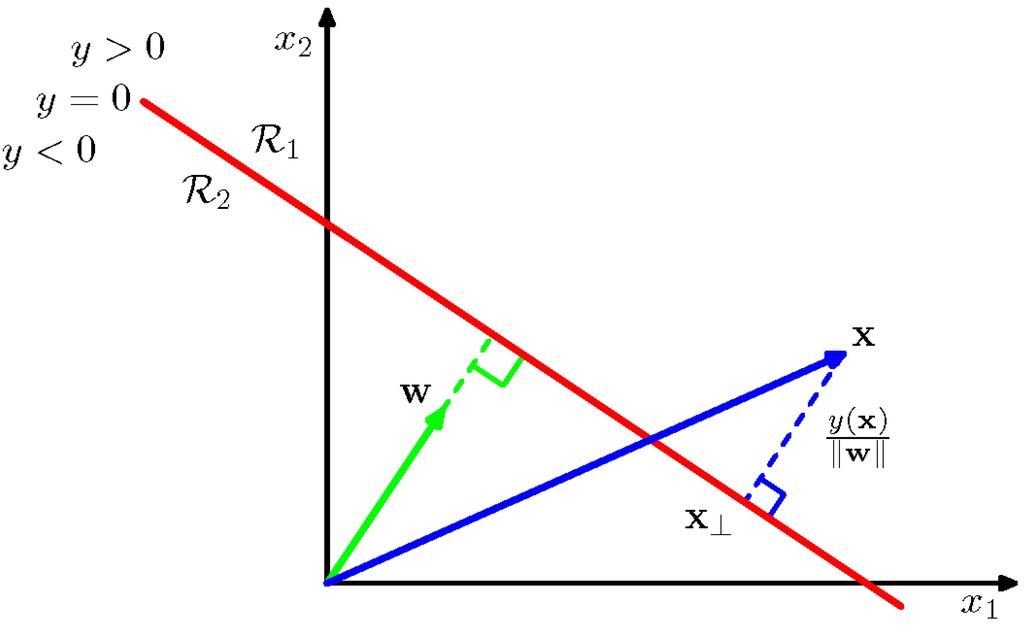
\includegraphics[width=0.7\linewidth]{fig8/lec816.jpg}
	\end{center}
\end{frame}



% 17
\begin{frame}[c]
	\frametitle{The distance from point $\mathbf{x}$𝒙to the hyperplane is 𝑦$y(\mathbf{x})/||\mathbf{w}||$}
	\begin{itemize}
		\item Consider a point $\mathbf{x}$ and its projection onto the hyperplane $\mathbf{x}_{\bot}$ so that $\mathbf{x}=\mathbf{x}_{\bot}+r\dfrac{\mathbf{w}}{||\mathbf{w}||}$
		\item We want to find $r$, the distance to the hyperplane
		\item Multiply both sides by $\mathbf{w}^T$ and add $b$
		      \[
			      \mathbf{w}^T\mathbf{x}+b=
			      \mathbf{w}^T\mathbf{x}_{\bot} +b+r\dfrac{||\mathbf{w}||^2}{||\mathbf{w}||}
		      \]
		      \[
			      y(\mathbf{x})=y(\mathbf{x}_{\bot})+r||\mathbf{w}||
		      \]
		      \[
			      r=\dfrac{y(\mathbf{x})}{||\mathbf{w}||}
		      \]
	\end{itemize}
\end{frame}



% 18
\begin{frame}[c]
	\frametitle{The distance from point $\mathbf{x}$𝒙to the hyperplane is $y(\mathbf{x})/||\mathbf{w}||$}
	\begin{center}
		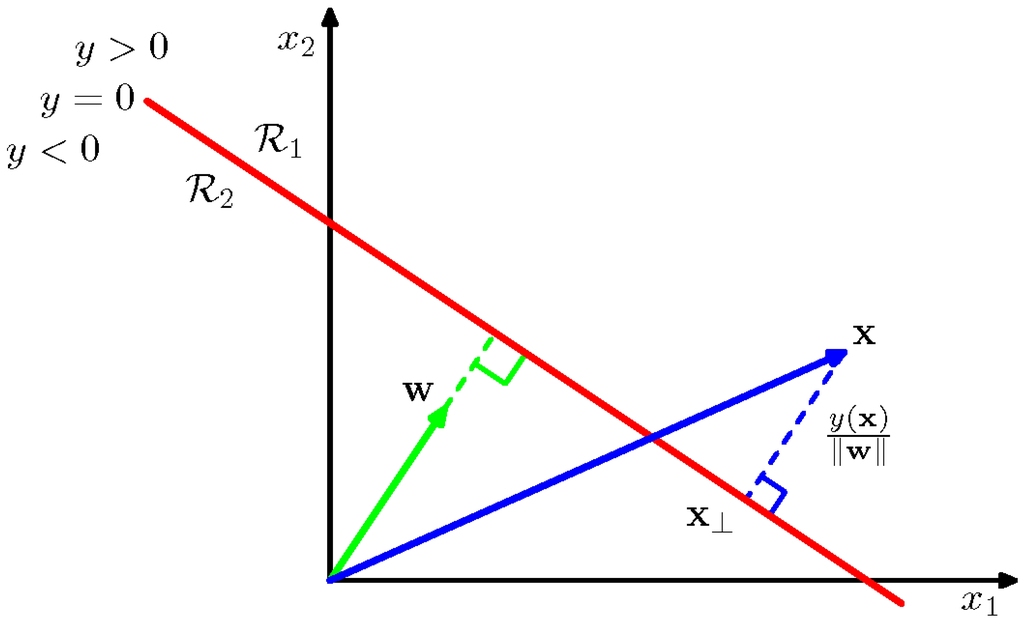
\includegraphics[width=0.7\linewidth]{fig8/lec818.jpg}
	\end{center}
\end{frame}


% 19
\begin{frame}[c]
	\frametitle{The maximum margin hyperplane is farthest from all of the data points}
	\begin{center}
		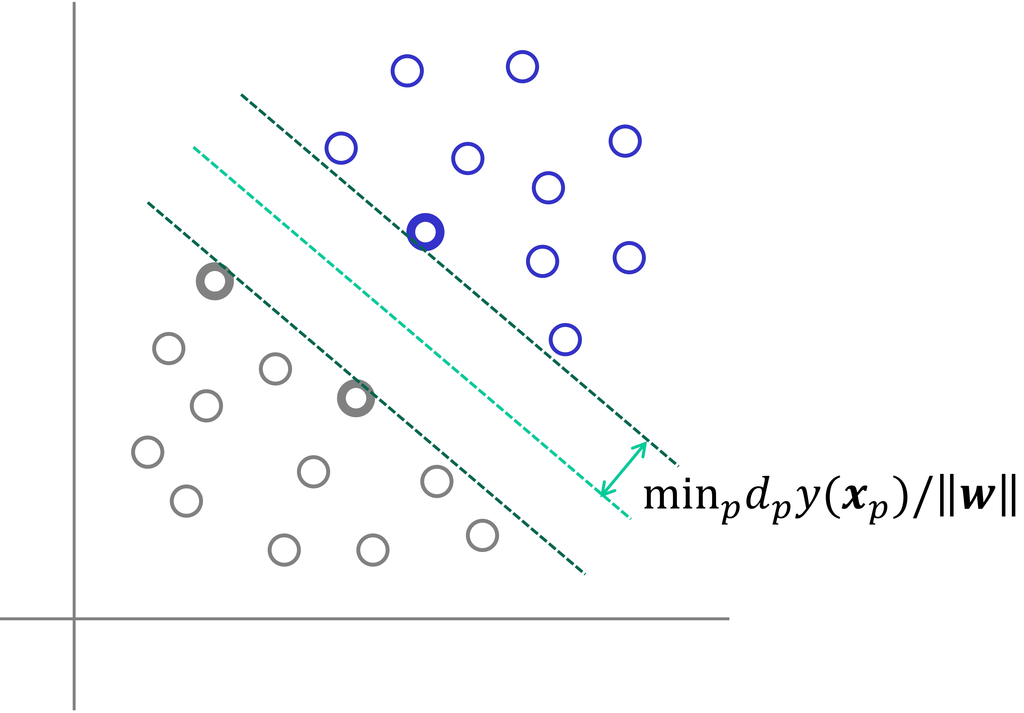
\includegraphics[width=0.7\linewidth]{fig8/lec819.jpg}
	\end{center}
\end{frame}


% 20
\begin{frame}[c]
	\frametitle{The maximum margin hyperplane is farthest from all of the data points}
	\begin{itemize}
		\item The margin is defined as
		      \[
			      \begin{array}{r@{~}l}
				      \alpha= & \min_pd_p\dfrac{y(\mathbf{x}_p)}{||\mathbf{w}||}  \\
				      =       & \dfrac{1}{||\mathbf{w}||}\min_pd_py(\mathbf{x}_p)
			      \end{array}
		      \]
		\item We want to find $\mathbf{w}$ and  that maximize the margin $\argmax_{\mathbf{w},b}\dfrac{1}{||\mathbf{w}||} \min_pd_py(\mathbf{x}_p)$
		\item Solving this problem is hard as it is written
	\end{itemize}
\end{frame}

% 21
\begin{frame}[c]
	\frametitle{We are free to choose a rescaling of $\mathbf{w}$}
	\begin{itemize}
		\item If we replace $\mathbf{w}$ by $a\mathbf{w}$ and $b$ with $ab$
		\item Then the margin is unchanged
		      \[
			      \min\nolimits_pd_p\dfrac{a\mathbf{w}^T\mathbf{x}_p+ab}{a||\mathbf{w}||}=
			      \min\nolimits_pd_p
			      \dfrac{\mathbf{w}^T\mathbf{x}_p+b}{||\mathbf{w}||}
		      \]
		\item So choose $a$ such that $\min_pd_p(a\mathbf{w}^T\mathbf{x}_p+ab)=1$
		\item Which means that for all points
		      \[
			      d_p(\mathbf{w}^T\mathbf{x}_p+b)\geqslant{}1
		      \]
	\end{itemize}
\end{frame}


% 22
\begin{frame}[c]
	\frametitle{Maximum margin constrained optimization problem}
	\begin{itemize}
		\item Then the maximum margin optimization becomes
		      \[
			      \begin{array}{c}
				      {\argmax}_{\mathbf{w},b}\dfrac{1}{||\mathbf{w}||} \min_pd_py(\mathbf{x}_p) \\
				      = {\argmax}_{\mathbf{w},b}\dfrac{1}{||\mathbf{w}||}
			      \end{array}
		      \]
		\item With the constraints $d_p(\mathbf{w}^T\mathbf{x}_p+b)\geqslant{}1$
	\end{itemize}
\end{frame}

% 23
\begin{frame}[c]
	\frametitle{Maximum margin constrained optimization problem}
	\begin{itemize}
		\item Which is equivalent to \\
		      $\argmin_{\mathbf{w},b}$ $\dfrac{1}{2}||\mathbf{w}||^2$, subject to $d_p(\mathbf{w}^T\mathbf{x}_p+b)\geqslant{}1$
		\item This is a well studied type of problem
		      \begin{itemize}
			      \item A quadratic program with linear inequality constraints
		      \end{itemize}
	\end{itemize}
\end{frame}



% 24
\begin{frame}[c]
	\frametitle{Detour: Lagrange multipliers solve constrained optimization problems}
	\begin{itemize}
		\item Want to maximize a function $f(x_1,x_2)$
		\item Subject to the equality constraint $g(x_1,x_2)= 0$
		\item Could solve $g(x_1,x_2)= 0$ for $x_1$ in terms of $x_2$
		      \begin{itemize}
			      \item But that is hard to do in general (i.e., on computers)
		      \end{itemize}
		\item Or could use Lagrange multipliers
		      \begin{itemize}
			      \item Which are easier to use in general (i.e., on computers)
		      \end{itemize}
	\end{itemize}
\end{frame}


% 25
\begin{frame}[c]
	\frametitle{Lagrange multipliers with general $\mathbf{x}$}
	\begin{itemize}
		\item In general, we can write
		      \[
			      \max\nolimits_x f(\mathbf{x})~\text{subject~to}~g(\mathbf{x})=0
		      \]
		\item Constraint $g(\mathbf{x})= 0$ defines a $D− 1$ dimensional surface for $D$ dimensional $\mathbf{x}$
	\end{itemize}
\end{frame}


% 26
\begin{frame}[c]
	\frametitle{Example: Maximize $f(\mathbf{x})=1-x_1^2-x_2^2$ subject to $g(\mathbf{x})=x_1+x_2-1=0$}
	\begin{center}
		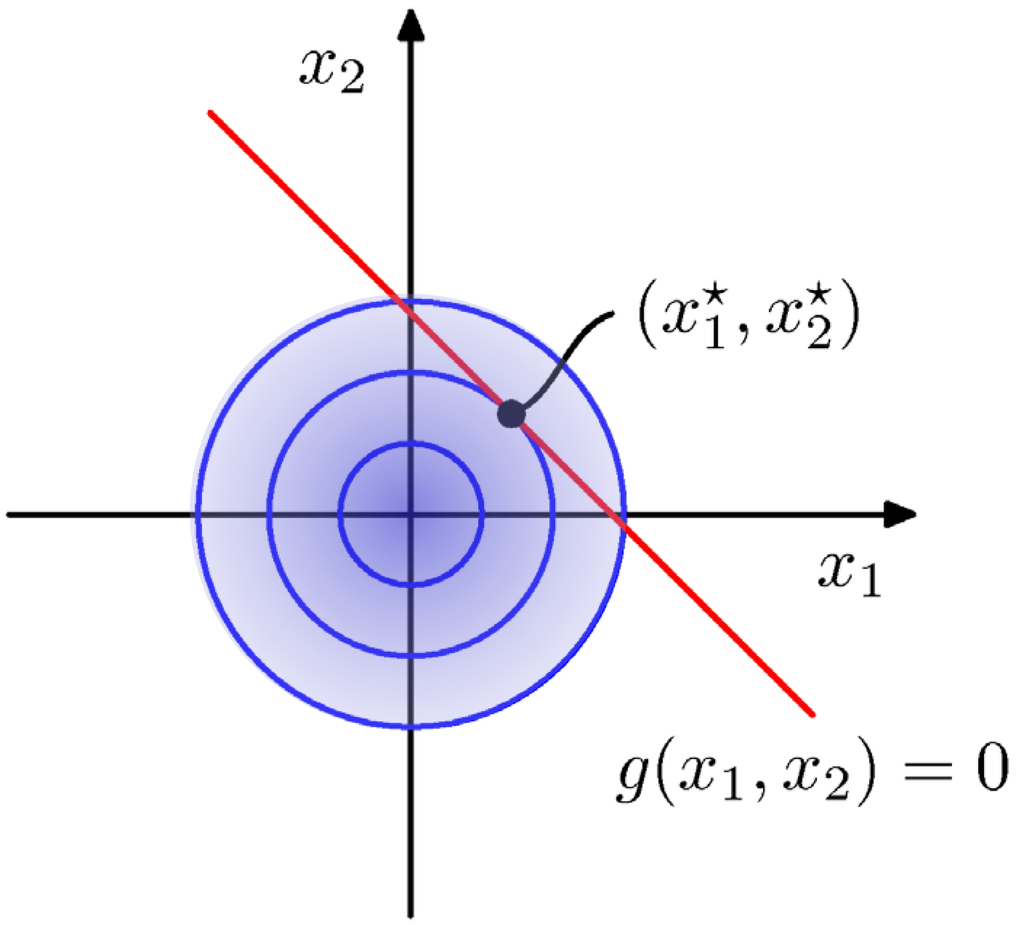
\includegraphics[width=0.7\linewidth]{fig8/lec826.jpg}
	\end{center}
\end{frame}


% 27
\begin{frame}[c]
	\frametitle{Gradients of $g$ and $f$ are orthogonal to surface at solution point}
	\begin{center}
		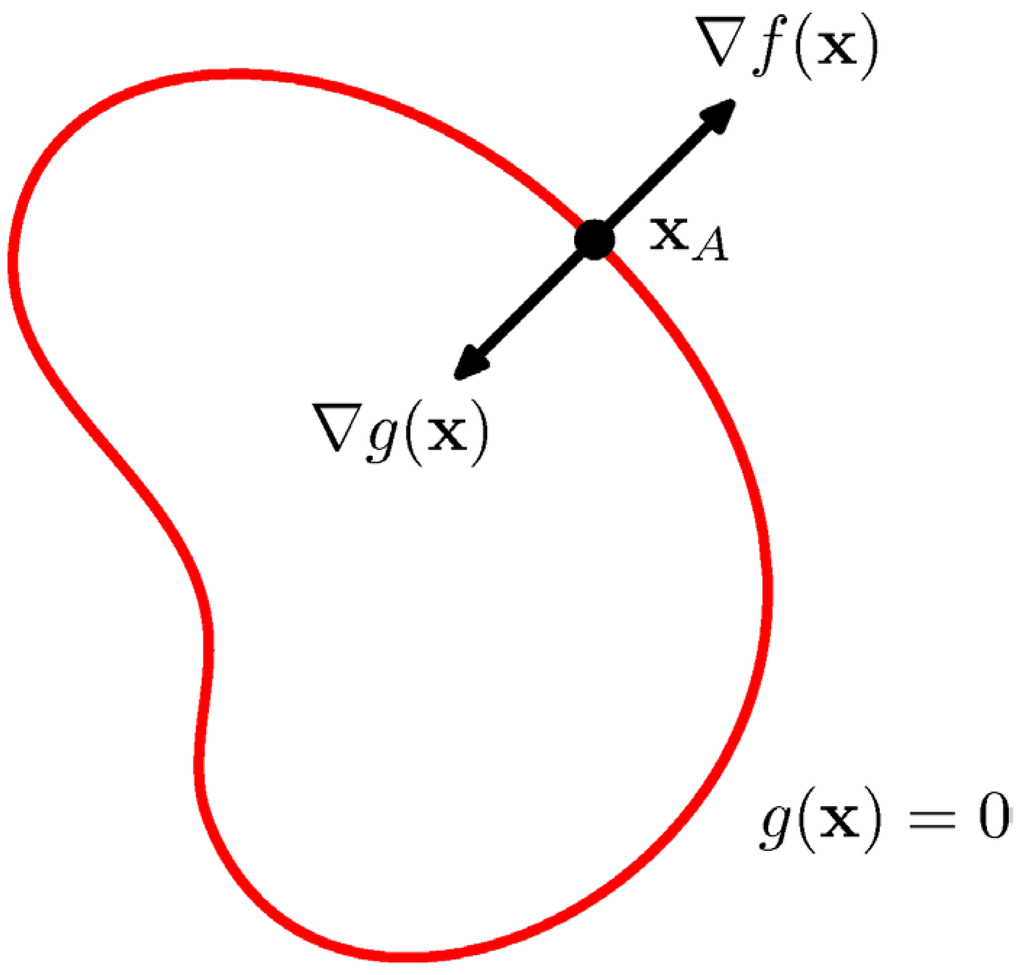
\includegraphics[width=0.65\linewidth]{fig8/lec827.jpg}
	\end{center}
\end{frame}



% 28
\begin{frame}[c]
	\frametitle{Gradients of $g$ and $f$ are orthogonal to surface at maximum of $f$}
	\begin{itemize}
		\item For $g$ because on all points on the surface $g(\mathbf{x})=0$
		\item For $f$ because if it wasn't, you could move along the surface in the direction of the gradient to find a better maximum
		\item Thus $\nabla f$ and $\nabla g$ parallel.    
			\begin{itemize}
				\item \red{If $g$ is inequality constraint}, $\nabla f$ and $\nabla g$ are of oppsite direction.
				\item If $g$ is equality constraint, we only know that they are parallel. 
			\end{itemize} 
		\item And there must exist a scalar $\lambda$ such that
		      \[
			      \nabla f+\lambda \nabla g=0
		      \]
	\end{itemize}
\end{frame}

% 29
\begin{frame}[c]
	\frametitle{The Lagrangian function captures the constraints on $x$ and on the gradients}
	\[
		L(\mathbf{x},\lambda)=f(\mathbf{x})+\lambda g(\mathbf{x})
	\]
	\begin{itemize}
		\item Setting gradient of $L$ with respect to $\mathbf{x}$ to 0 gives
		      \[
			      \nabla f+\lambda \nabla g=0
		      \]
		\item Setting partial of $L$ with respect to $\lambda$ to 0 gives
		      \[
			      g(\mathbf{x})=0
		      \]
		\item Thus stationary points of $L$ solve the constrained optimization problem
	\end{itemize}
\end{frame}



% 30
\begin{frame}[c]
	\frametitle{Example: Maximize $f(\mathbf{x})=1-x_1^2-x_2^2$ subject to $g(\mathbf{x})=x_1+x_2-1=0$}
	\begin{center}
		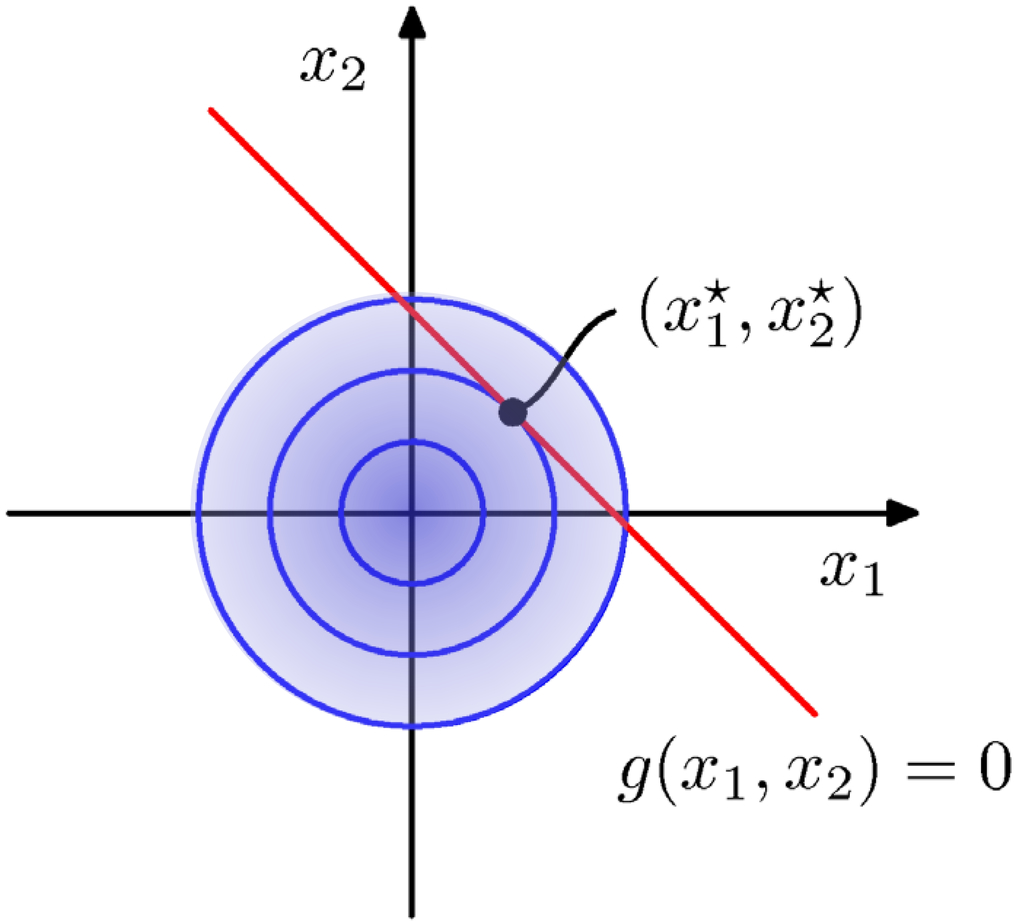
\includegraphics[width=0.65\linewidth]{fig8/lec830.jpg}
	\end{center}
\end{frame}


% 31
\begin{frame}[c]
	\frametitle{Example: Maximize $f(\mathbf{x})=1-x_1^2-x_2^2$ subject to $g(\mathbf{x})=x_1+x_2-1=0$}
	\begin{itemize}
		\item So the Lagrangian function is
		      \[
			      \begin{array}{r@{~}l}
				      L(\mathbf{x},\lambda)= & f(\mathbf{x})+\lambda g(\mathbf{x}) \\
				      =                      & 1-x_1^2-x_2^2+\lambda(x_1+x_2-1)
			      \end{array}
		      \]
		\item The conditions for $L$ to be stationary are
		      \[
			      \begin{array}{l@{~}l}
				      \partial L/\partial x_1=-2x_1+\lambda=0 \\
				      \partial L/\partial x_2=-2x_2+\lambda=0 \\
				      \partial L/\partial \lambda=x_1+x_2-1=0 \\
			      \end{array}
		      \]
		\item Can solve to find $\lambda=1,x_1=x_2=\dfrac{1}{2}$
	\end{itemize}
\end{frame}


% 32
\begin{frame}[c]
	\frametitle{Lagrange multipliers can also be used with inequality constraints $g(\mathbf{x})\geqslant{}0$}
	\begin{center}
		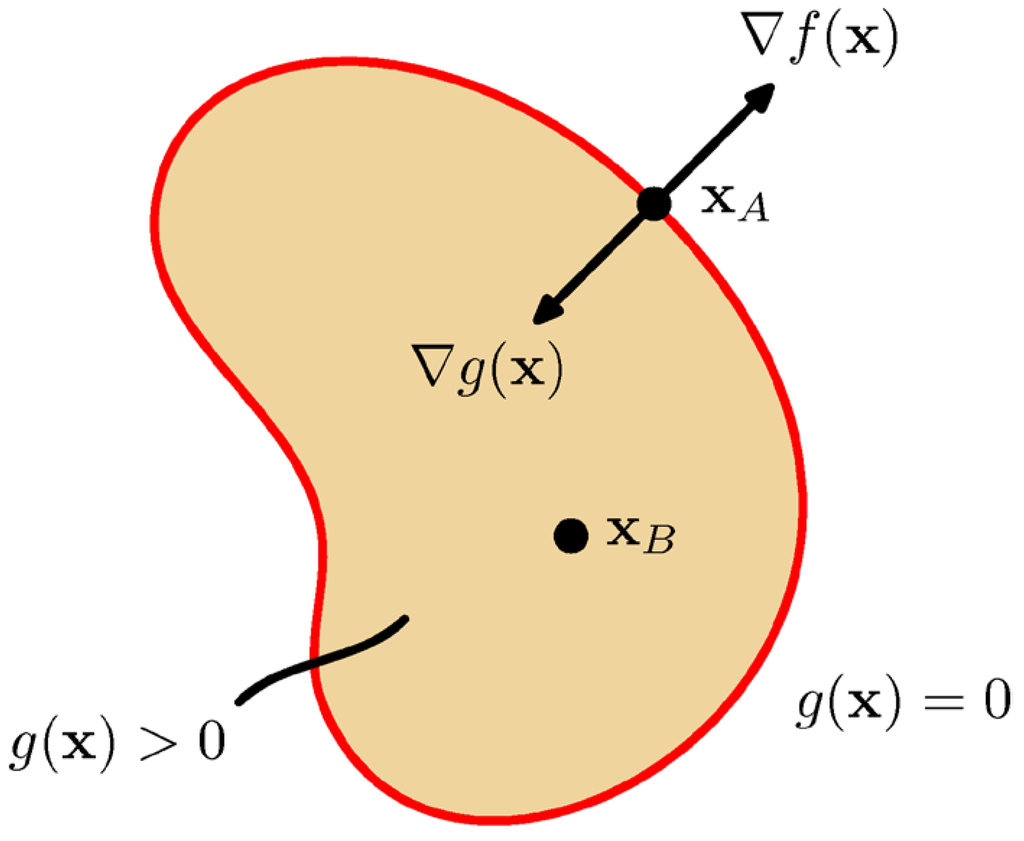
\includegraphics[width=0.65\linewidth]{fig8/lec832.jpg}
	\end{center}
\end{frame}


% 33
\begin{frame}[c]
	\frametitle{Lagrange multipliers can also be used with inequality constraints $g(\mathbf{x})\geqslant{}0$}
	\begin{itemize}
		\item Now two kinds of solutions:
		\item If $g(\mathbf{x})> 0$, then the solution only depends on $f(\mathbf{x})$
		      \begin{itemize}
			      \item Inside constraint surface with $\nabla f= 0$
			      \item Stationary point of $L(\mathbf{x},𝜆\lambda)$ with $\lambda= 0$
			      \item Constraint $g(\mathbf{x})$ is said to be inactive
		      \end{itemize}
		\item If $g(\vx)= 0$, then same as before (with equality constraint)
		      \begin{itemize}
			      \item On boundary of constraint surface with $\nabla f$ pointing out
			      \item Stationary point of $L(\mathbf{x},\lambda)$ with $\lambda> 0$
			      \item Constraint $g(\mathbf{x})$ is said to be active
		      \end{itemize}

	\end{itemize}
\end{frame}


% 34
\begin{frame}[c]
	\frametitle{Lagrange multipliers can also be used with inequality constraints $g(\mathbf{x})\geqslant{}0$}
	\begin{itemize}
		\item In either case, $\lambda g(\mathbf{x})=0$
		\item Thus maximizing $f(\mathbf{x})$ subject to $g(\mathbf{x})\geqslant{}0$ is obtained by optimizing $L(\mathbf{x},\lambda)$ \wrt $\mathbf{x}$ and $\lambda$ subject to
		      \[
			      \begin{array}{cc}
				      g(\mathbf{x})         & \geqslant{}0 \\
				      \lambda               & \geqslant{}0 \\
				      \lambda g(\mathbf{x}) & =0
			      \end{array}
		      \]
		\item These are known as the Karush-Kuhn-Tucker (KKT) conditions
	\end{itemize}
\end{frame}


% 35
\begin{frame}[c]
	\frametitle{Example: Maximize $f(\mathbf{x})=1-x_1^2-x_2^2$ subject to $g(\mathbf{x})=x_1+x_2-1\geqslant{}0$}
	\begin{center}
		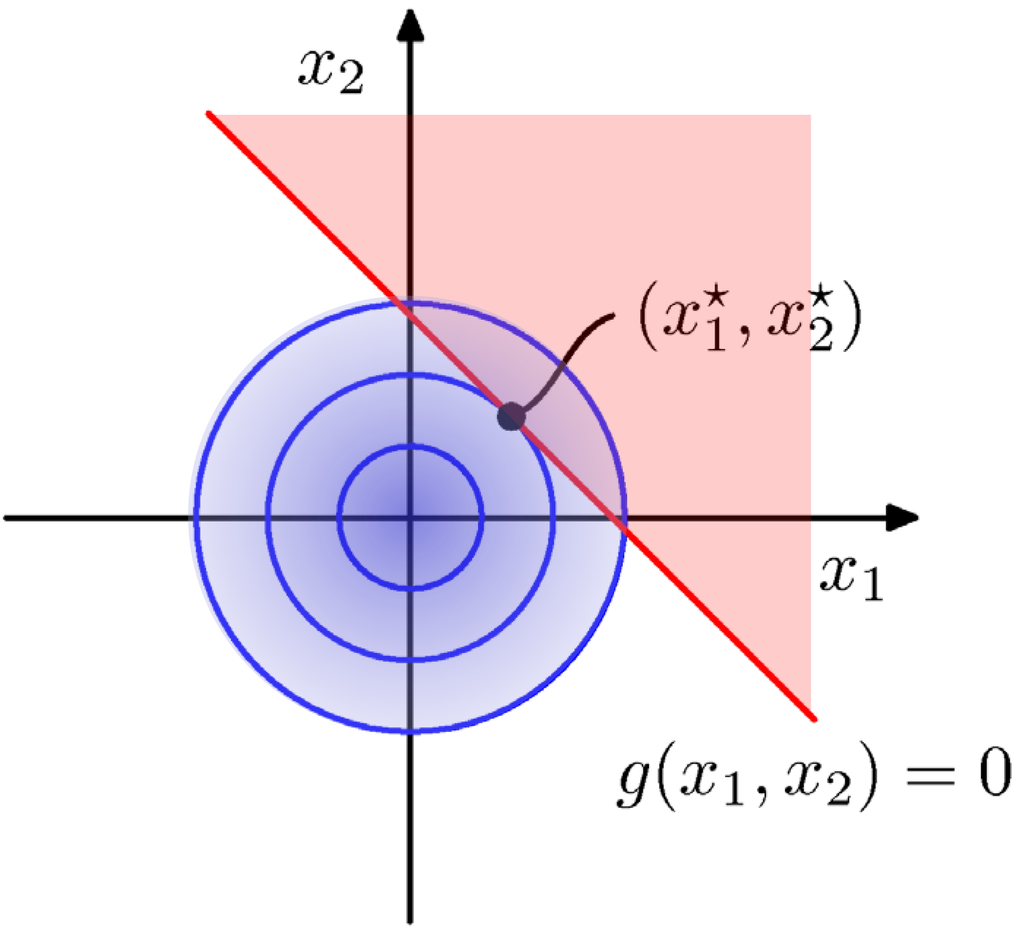
\includegraphics[width=0.65\linewidth]{fig8/lec835.jpg}
	\end{center}
\end{frame}


% 36
\begin{frame}[c]
	\frametitle{Example: Maximize $f(\mathbf{x})=1-x_1^2-x_2^2$ subject to $g(\mathbf{x})=x_1+x_2-1\geqslant{}0$}
	\begin{itemize}
		\item So the Lagrangian function is
		      \[
			      L(\mathbf{x},\lambda)=1-x_1^2-x_2^2+\lambda(x_1+x_2-1)
		      \]
		\item The conditions for $L$ to be stationary are
		      \[
			      \begin{array}{r@{~}l}
				      \partial L/\partial x_1=-2x_1+\lambda=0 \\
				      \partial L/\partial x_2=-2x_2+\lambda=0 \\
				      \partial L/\partial \lambda=x_1+x_2-1=0 \\
			      \end{array}
		      \]
		\item Can solve to find $\lambda=1,x_1=x_2=\dfrac{1}{2}$
		      \begin{itemize}
			      \item Which still satisfies KKT conditions
		      \end{itemize}
	\end{itemize}
\end{frame}


% 37
\begin{frame}[c]
	\frametitle{Example: Maximize $f(\mathbf{x})=1-x_1^2-x_2^2$ subject to $g(\mathbf{x})=-x_1-x_2+1\geqslant{}0$}
	\begin{center}
		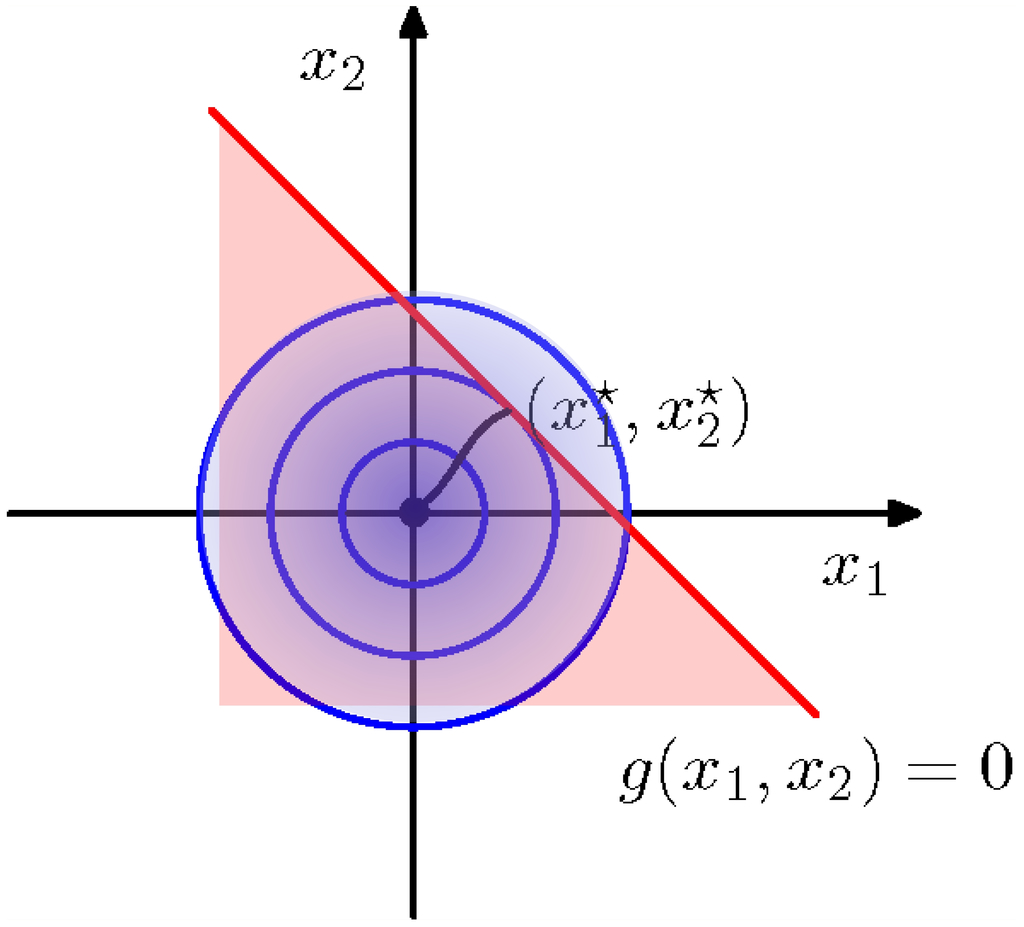
\includegraphics[width=0.65\linewidth]{fig8/lec837.jpg}
	\end{center}
\end{frame}


% 38
\begin{frame}[c]
	\frametitle{Example: Maximize $f(\mathbf{x})=1-x_1^2-x_2^2$ subject to $g(\mathbf{x})=-x_1-x_2+1\geqslant{}0$}
	\begin{itemize}
		\item So the Lagrangian function is
		      \[
			      L(\mathbf{x},\lambda)=1-x_1^2-x_2^2+\lambda(-x_1-x_2+1)
		      \]
		\item The conditions for $L$ to be stationary are
		      \[
			      \begin{array}{r@{~}l}
				      \partial L/\partial x_1=-2x_1-\lambda=0 \\
				      \partial L/\partial x_2=-2x_2-\lambda=0 \\
				      \partial L/\partial \lambda=x_1+x_2-1=0 \\
			      \end{array}
		      \]
		\item Can solve to find $\lambda=-1$
		      \begin{itemize}
			      \item which does not satisfy KKT condition $\lambda \geqslant{}0$
		      \end{itemize}
		\item Instead use unconstrained solution $x_1=x_2=0$
		      \begin{itemize}
			      \item which does satisfy KKT conditions
		      \end{itemize}
	\end{itemize}
\end{frame}


% 39
\begin{frame}[c]
	\frametitle{Multiple constraints each get their own Lagrange multiplier}
	\begin{itemize}
		\item Maximize $f(\mathbf{x})$ subject to $h_j(\mathbf{x})= 0$ and $g_i(\vx)\geqslant{}0$
		\item Leads to the Lagrangian function
		      \[
			      L(\mathbf{x,\lambda,\nu})=f(\mathbf{x})+\sum_i \lambda_ig_i(\mathbf{x})+\sum_ju_jh_j(\mathbf{x})
		      \]
		\item Still solve for $\nabla L(\mathbf{x,\lambda,\nu})= 0$
		\item Trickier in general to figure out which $h_j(\mathbf{x})$ constraints should be active
	\end{itemize}
\end{frame}



% 40
\begin{frame}[c]
	\frametitle{Minimizing $f(\mathbf{x})$ with an inequality constraint requires a slightly different Lagrange}
	\begin{itemize}
		\item Subject to
		      \[
			      g(\mathbf{x}) \le 0
		      \]

		\item Minimize \wrt $\mathbf{x}$
		      \[
			      L(\mathbf{x},\lambda)=f(\mathbf{x})+\lambda g(\mathbf{x})
		      \]
	\end{itemize}
\end{frame}


% 41
\begin{frame}[c]
	\frametitle{Summary of Lagrange multipliers with multiple inequality constraints}
	\begin{itemize}
		\item Goal: maximize $f(\mathbf{x})$ subject to $g_i(\mathbf{x})\geqslant{} 0$
		\item Write down Lagrangian function
		      \[
			      L(\mathbf{x},\lambda)=f(x)+\sum_i\lambda_ig_i(\mathbf{x})
		      \]
		\item Find points where $\nabla L(\mathbf{x},\lambda)= 0$
		\item Keep points that satisfy constraints $g_x(\mathbf{x})\geqslant{}0$
		\item Figure out which KKT conditions should be active
		      \begin{itemize}
			      \item Don't need to try all $2^I$ combinations for SVMs
			      \item Because $f(\mathbf{x})$ and $g(\mathbf{x})$ form a ``quadratic program''
		      \end{itemize}
	\end{itemize}
\end{frame}

\begin{frame}
	{Recap: Lagrange dual problem}
	\begin{block}{Primal Problem}
		\vspace{-1em}
		\begin{equation}
			\begin{aligned}
				\max_\vx   \quad    & f(\vx)                            \\
				\textrm{s.t.} \quad & g_i(\vx) \ge 0, \quad i=1,\dots,m \\
				                    & h_j(\vx) =0 ,\quad j=1,\dots, p   \\
				                    & \vx \in D                         \\
			\end{aligned}
		\end{equation}
	\end{block}

	\begin{block}{Dual Problem}
		\vspace{-1em}
		\begin{equation}
			\begin{aligned}
				\min_{\vlambda, \vnu}   \quad    & \tilde{L}( \vlambda, \vnu) \\
				\textrm{s.t.} \quad & \vlambda \ge 0             \\
			\end{aligned}
		\end{equation}
		, where
		\vspace{-1em}
		\begin{equation*}
			\tilde{L}(\vlambda, \vnu ) =  \sup_{\vx \in D} L(\vx, \vlambda, \vnu)
			= \sup_{\vx \in D} \left\{ f(\vx)+  \sum_i \lambda_i g_i(\vx) + \sum_j \nu_j h_j(\vx) \right\}
		\end{equation*}
	\end{block}
	% \end{columns}
\end{frame}

\begin{frame}
	{Recap: Lagrange dual problem}
	\begin{block}{Primal Problem}
		\vspace{-1em}
		\begin{equation}
			\begin{aligned}
				\min_\vx   \quad    & f(\vx)                           \\
				\textrm{s.t.} \quad & g_i(\vx) \le 0,\quad i=1,\dots,m \\
				                    & h_j(\vx) =0 ,\quad j=1,\dots, p  \\
				                    & \vx \in D                        \\
			\end{aligned}
		\end{equation}
	\end{block}
	\begin{block}{Dual Problem}
		\vspace{-1em}
		\begin{equation}
			\begin{aligned}
				\max_{\vlambda, \vnu}   \quad    & \tilde{L}( \vlambda, \vnu) \\
				\textrm{s.t.} \quad & \vlambda \ge 0             \\
			\end{aligned}
		\end{equation}
		, where
		\vspace{-1em}
		\begin{equation*}
			\tilde{L}(\vlambda, \vnu ) =  \inf_{\vx \in D} L(\vx, \vlambda, \vnu)
			= \inf_{\vx \in D} \left\{ f(\vx)+  \sum_i \lambda_i g_i(\vx) + \sum_j \nu_j h_j(\vx) \right\}
		\end{equation*}
	\end{block}
	% \end{columns}
\end{frame}

\begin{frame}
	{Example}

	\begin{block}{Primal Problem}
		\vspace{-1em}
		\begin{equation}
			\begin{aligned}
				\min_x \quad        & \vc^T \vx               \\
				\textrm{s.t.} \quad & \mA_1 \vx \succeq \vb_1 \\
				                    & \mA_2 \vx = \vb_2       \\
				                    & \vx \succeq 0           \\
			\end{aligned}
		\end{equation}
	\end{block}
	\pause
	\begin{block}{Dual Problem}
		\vspace{-1em}
		\begin{equation*}
			\begin{aligned}
				\tilde{L}(\vlambda, \vnu ) & = \inf_{\vx \in D} L(\vx, \vlambda, \vnu)                                                                                \\
				                           & = \inf_{\vx \succeq 0} \left\{ (\vc^T - \vlambda^T \mA_1 - \vnu^T \mA_2 ) \vx + \vlambda^T \vb_1 + \vnu^T \vb_2 \right\} \\
				                           & = \begin{cases}
					\vlambda^T \vb_1 + \vnu^T \vb_2 & \vc^T - \vlambda^T \mA_1 - \vnu^T \mA_2 \succeq 0 \\
					-\infty                         & \vc^T - \vlambda^T \mA_1 - \vnu^T \mA_2 \prec 0   \\
				\end{cases}                                                                                             \\
			\end{aligned}
		\end{equation*}
	\end{block}
\end{frame}


\begin{frame}
	{Example}
	\begin{block}{Dual Problem}
		\vspace{-1em}
		\begin{equation*}
			\begin{aligned}
				\tilde{L}(\vlambda, \vnu ) & = \inf_{\vx \in D} L(\vx, \vlambda, \vnu)                                                                                \\
				                           & = \inf_{\vx \succeq 0} \left\{ (\vc^T - \vlambda^T \mA_1 - \vnu^T \mA_2 ) \vx + \vlambda^T \vb_1 + \vnu^T \vb_2 \right\} \\
				                           & = \begin{cases}
					\vlambda^T \vb_1 + \vnu^T \vb_2 & \vc^T - \vlambda^T \mA_1 - \vnu^T \mA_2 \succeq 0 \\
					-\infty                         & \vc^T - \vlambda^T \mA_1 - \vnu^T \mA_2 \prec 0   \\
				\end{cases}                                                                                             \\
			\end{aligned}
		\end{equation*}

		\begin{equation}
			\begin{aligned}
				\max_{\vlambda, \vnu} \quad        & \vlambda^T \vb_1 + \vnu^T \vb_2               \\
				\textrm{s.t.} \quad & \vlambda^T \mA_1 - \vnu^T \mA_2 \preceq \vc^T \\
				                    & \vlambda \succeq 0                            \\
			\end{aligned}
		\end{equation}

	\end{block}
\end{frame}

\begin{frame}
	{LP as a special case}
	\begin{columns}
		\column{.5\textwidth}
		\begin{block}{Primal}
			\begin{equation}
				\begin{aligned}
					\min_x \quad        & c^T x    \\
					\textrm{s.t.} \quad & Ax \ge b \\
					                    & x \ge 0  \\
				\end{aligned}
			\end{equation}
		\end{block}
		\pause
		\column{.5\textwidth}
		\begin{block}{Dual}
			\begin{equation}
				\begin{aligned}
					\red{\max}_\lambda \quad        & b^T \lambda       \\
					\textrm{s.t.} \quad & A^T \lambda \le c \\
					                    & \lambda \ge 0     \\
				\end{aligned}
			\end{equation}
		\end{block}
	\end{columns}
	\begin{equation*}
		\begin{aligned}
			\tilde{L}(\lambda) & = \inf_{x \ge 0 } L(x, \lambda)                                           \\
			                   & = \inf_{x \ge 0 } \left\{ (c^T - \lambda^T A ) x + \lambda ^T b  \right\} \\
			                   & = \begin{cases}
				\lambda^T b & \lambda^T A \le c^T \\
				-\infty     & \lambda^T A > c^T   \\
			\end{cases}                                              \\
		\end{aligned}
	\end{equation*}
\end{frame}

\begin{frame}
	{Example for LP Duality}
	Q1: Raw materials A1, A2 and A3 will be made into products X and Y. The ingredients and requirements for products are show in table.
	\begin{table}
		\begin{tabular}{cccc}
			\hline
			\multirow{2}{*}{Ingredients} & \multicolumn{2}{c}{Products} & \multirow{2}{*}{Minimal requirements}       \\ \cline{2-3}
			                             & X                            & Y                                     &     \\  \hline \hline
			A1                           & 0.1                          & 0.15                                  & 1   \\
			A2                           & 1.7                          & 0.75                                  & 7.5 \\
			A3                           & 1.2                          & 1.3                                   & 10  \\ \hline
			cost                         & 3                            & 2                                     &     \\ \hline
		\end{tabular}
	\end{table}

\end{frame}


\begin{frame}{Example for LP Duality}
	\begin{table}
		\begin{tabular}{cccc}
			\hline
			\multirow{2}{*}{Ingredients} & \multicolumn{2}{c}{Products} & \multirow{2}{*}{Minimal requirements}       \\ \cline{2-3}
			                             & X                            & Y                                     &     \\  \hline \hline
			A1                           & 0.1                          & 0.15                                  & 1   \\
			A2                           & 1.7                          & 0.75                                  & 7.5 \\
			A3                           & 1.2                          & 1.3                                   & 10  \\ \hline
			cost                         & 3                            & 2                                     &     \\ \hline
		\end{tabular}
	\end{table}

	\begin{equation*}
		\begin{aligned}
			\min \quad          & z=3x_1 +2x_2               \\
			\textrm{s.t.} \quad & 0.1x_1 + 0.15x_2 \ge 1     \\
			                    & 1.7 x_1 + 0.75 x_2 \ge 7.5 \\
			                    & 1.2x_1 + 1.3x_2 \ge 10     \\
			                    & x_1, x_2	 \ge 0             \\
		\end{aligned}
	\end{equation*}

\end{frame}

\begin{frame}
	{Example for LP Duality}
	Q1: Raw materials A1, A2 and A3 will be made into products X and Y. The ingredients and requirements for products are show in table.

	Q2: The company is selling raw materials A1, A2 and A3. How to make the price for A1, A2 and A3 to  maximize profit of the company and make sure the price is acceptable comparing to products X and Y?

\end{frame}


\begin{frame}
	{Example for LP Duality}
	\begin{table}
		\begin{tabular}{cccc}
			\hline
			\multirow{2}{*}{Ingredients} & \multicolumn{2}{c}{Products} & \multirow{2}{*}{Minimal requirements}       \\ \cline{2-3}
			                             & X                            & Y                                     &     \\  \hline \hline
			A1                           & 0.1                          & 0.15                                  & 1   \\
			A2                           & 1.7                          & 0.75                                  & 7.5 \\
			A3                           & 1.2                          & 1.3                                   & 10  \\ \hline
			cost                         & 3                            & 2                                     &     \\ \hline
		\end{tabular}
	\end{table}
	\begin{equation*}
		\begin{aligned}
			\max \quad          & w= 1 y_1 + 7.5y_2 +10 y_3          \\
			\textrm{s.t.} \quad & 0.1 y_1 + 1.7 y_2 + 1.2 y_3 \le 3  \\
			                    & 0.15y_1 + 0.75 y_2 + 1.3 y_3 \le 2 \\
			                    & y_1,y_2,y_3 \ge 0                  \\
		\end{aligned}
	\end{equation*}
\end{frame}



\begin{frame}
	{Karush-Kuhn-Tucker (KKT) Conditions}

	\begin{block}{KKT conditions for differentiable $g_i$, $h_i$}
		\begin{itemize}
			\item Primal feasible: $g_i(x) \le 0, h_j(x) =0$
			\item Dual feasible: $\lambda \ge 0$
			\item Complementary slackness: $\lambda_i^* f_i(x^*) =0$
			\item Zero gradient of Lagrangian \wrt $x$
			      \[\nabla f_(x) + \sum_{i} \lambda_i \nabla g_i(x) + \sum_{j} \nu_j \nabla h_j(x) =0 \]
		\end{itemize}
	\end{block}

\end{frame}

\begin{frame}
	{KKT for LP}
	\begin{columns}
		\column{.5\textwidth}
		\begin{block}{Primal}
			\begin{equation} \label{eq:p}
				\begin{aligned}
					\min_x \quad        & c^T x    \\
					\textrm{s.t.} \quad & Ax \ge b \\
					                    & x \ge 0  \\
				\end{aligned}
			\end{equation}
		\end{block}
		\column{.5\textwidth}
		\begin{block}{Dual}
			\begin{equation} \label{eq:d}
				\begin{aligned}
					\red{\max}_\lambda \quad        & b^T \lambda       \\
					\textrm{s.t.} \quad & A^T \lambda \le c \\
					                    & \lambda \ge 0     \\
				\end{aligned}
			\end{equation}
		\end{block}
	\end{columns}
	\begin{theorem}[KKT for LP]
		If $x'$ is feasible for Primal Problem~\ref{eq:p} and $\lambda'$ is feasible for Dual Problem~\ref{eq:d} and $c^Tx' = b^T \lambda'$, then $x'$ and $\lambda'$ is optimal for   Problem~\ref{eq:p} and \ref{eq:d} respectively.
	\end{theorem}
\end{frame}

% 42
\begin{frame}[c]
	\frametitle{Back to SVMs: Maximum margin solution is a fixed point of the Lagrangian function}
	\begin{itemize}
		\item Recall, the maximum margin hyperplane is

		      $\argmin_{\mathbf{w},b} \dfrac{1}{2}||\mathbf{w}||^2$ subject to $d_p(\mathbf{w}^T \mathbf{x}_p+b)\geqslant{}1$
		      \begin{itemize}
			      \item Minimization of a quadratic function subject to multiple linear inequality constraints
		      \end{itemize}
		\item Will use Lagrange multipliers, $a_p$, to write Lagrangian function

		      $$L(\mathbf{w},b,\mathbf{a})=\dfrac{1}{2}||\mathbf{w}||^2-\sum_{p}a_p(d_p( \mathbf{w} ^T\mathbf{x}_p+b)-1)$$

		\item Note that $\mathbf{x}_p$ and $d_p$ are fixed for the optimization
	\end{itemize}
\end{frame}




\begin{frame}
	\begin{center}
		\chuhao Thank you! %\fontspec{LHANDW.TTF}
	\end{center}
\end{frame}
\end{document}
